\begin{figure}
	\begin{center}
		\begin{tikzpicture}[scale=1]
			\coordinate (O) at (0,0);

			\tikzmath{
						\tmax=5;	\ymax=2;
						\x0=.1;	\x1=\tmax/2;	\x2=\tmax-.5;
			}

			\draw [-latex] ($(O)+(-0.1,0)$) -- ($(O)+(\tmax,0)$) node [right] {t};
			\draw [-latex] ($(O)+(0,-0.1)$) -- ($(O)+(0,\ymax)$) node [left] {X(t)};

			\draw [dotted] ($(O)+(0,\ymax-.5)$) node [left] {$V_T$} -- ($(O)+(\tmax,\ymax-.5)$);

			\draw [-latex] ($(O)+(\x0,-.2)$) node [below] {Beginning} -- ($(O)+(\x0,0)$);
			\foreach \k in {0,...,5}{
				\tikzmath{
							\x = \x0;
							\y = 0.25 * rnd;}
				\draw ($(O)+(\x,\y)$) node {$\cdot$};
			};

			\draw [-latex] ($(O)+(\x1,-.2)$) node [below] {During simulation} -- ($(O)+(\x1,0)$);
			\foreach \k in {0,...,5}{
				\tikzmath{
							\x = \x1;
							\y = 0.25 * rnd + 0.5;}
				\draw ($(O)+(\x,\y)$) node {$\cdot$};
			};

			\draw [-latex] ($(O)+(\x2,-.2)$) node [below] {Near first spike} -- ($(O)+(\x2,0)$);
			\foreach \k in {0,...,5}{
				\tikzmath{
							\x = \x2;
							\y = .25 * rnd + 1.35;}
				\draw ($(O)+(\x,\y)$) node {$\cdot$};
			};
		\end{tikzpicture}
		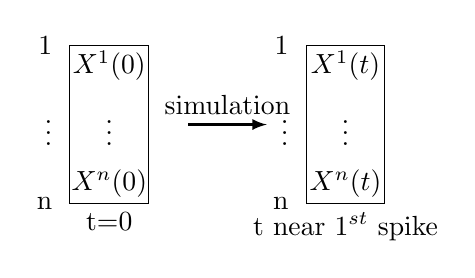
\begin{tikzpicture}[scale=1]
			\draw (0,0) rectangle (1,2);
			\node [left] at (-.1,2) {1};		\node at (.5,1.75) {$X^1(0)$};
			\node [left] at (-.1,1) {$\vdots$};	\node at (.5,1) {$\vdots$};
			\node [left] at (-.1,0) {n};		\node at (.5,.25) {$X^n(0)$};
			\node [below] at (.5,0) {t=0};
			
			\draw [thick,-latex] (1.5,1) -- (2.5,1) node [midway,above] {simulation};

			\draw (3,0) rectangle (4,2);
			\node [left] at (2.9,2) {1};		\node at (3.5,1.75) {$X^1(t)$};
			\node [left] at (2.9,1) {$\vdots$};	\node at (3.5,1) {$\vdots$};
			\node [left] at (2.9,0) {n};		\node at (3.5,.25) {$X^n(t)$};
			\node [below] at (3.5,0) {t near $1^{st}$ spike};
		\end{tikzpicture}
	\end{center}
	\caption{Illustration of the initialisation process, the state of the system is represented at different instants of the simulation (each dot is a neuron, x-absciss time and y-absciss the potential of the neuron).}
	\label{fig:init}
\end{figure}